\section{Work Environment Example}
TODO: esempio di deployment con immagine casa.

\begin{figure}[H]
	\begin{center}
		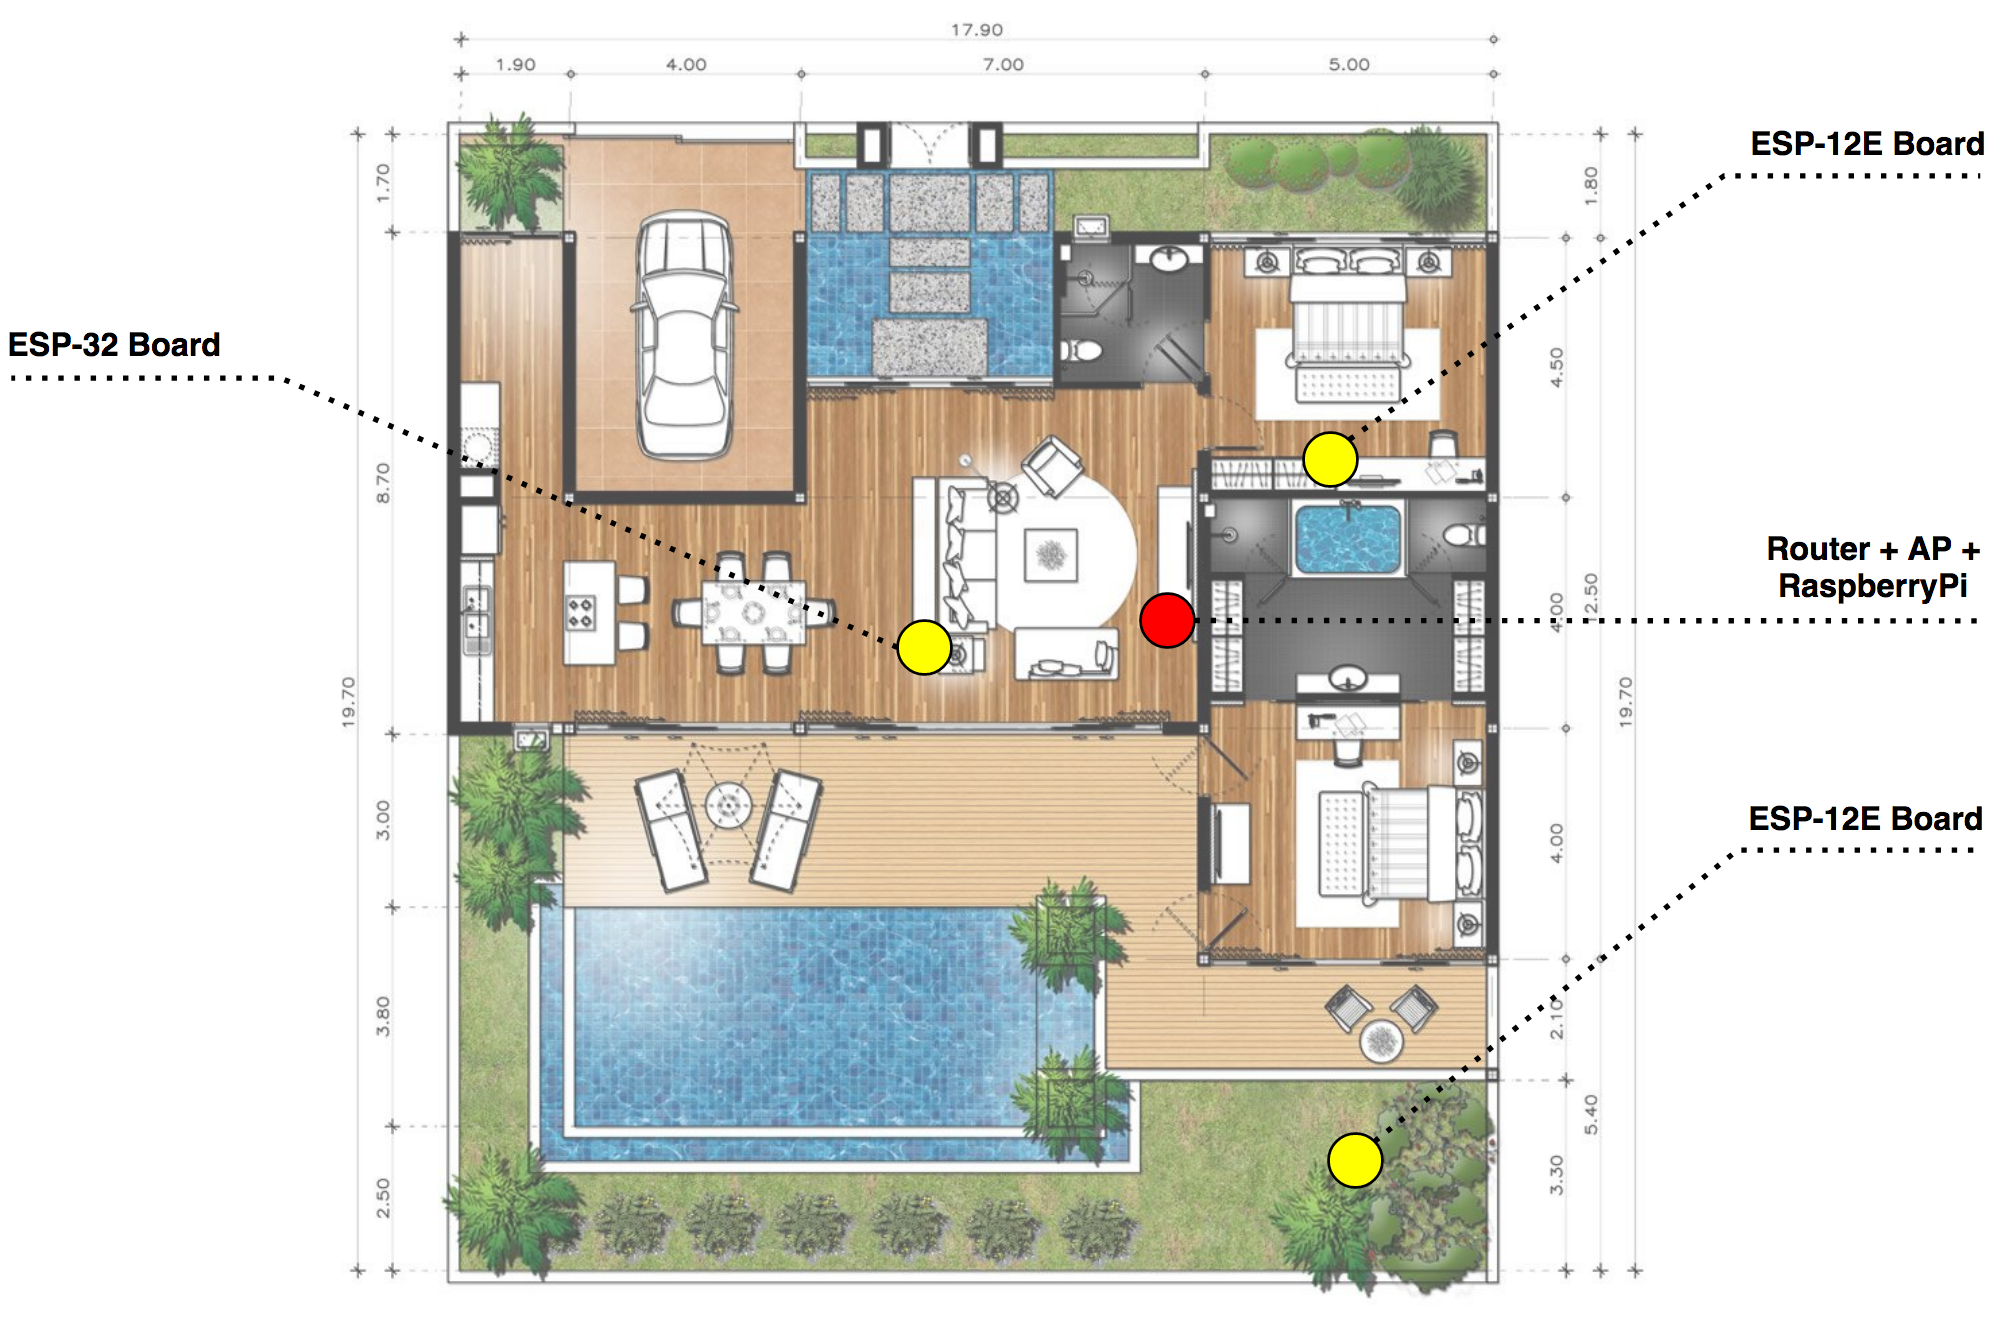
\includegraphics[width=\textwidth]{./pictures/blueprint_deployment.png}
		\caption{.}
		\label{blueprint_deployment}
	\end{center}
\end{figure}

TODO: aggiungere la Raspberry Pi alla figura.

\section{Future Extensions}
TODO: spiegare che è possibile collegare più di tre schede, diversi sensori e attuatori. Esempio: sensori di pressione. E' anche possibile collegare pannelli solari per ricavare energia in caso di alimentazione a batteria.